\documentclass{standalone}
\usepackage{tikz}
\usetikzlibrary{patterns, positioning}
\usepackage[sfdefault]{ClearSans} %% option 'sfdefault' activates Clear Sans as the default text font
\usepackage[T1]{fontenc}

\begin{document}
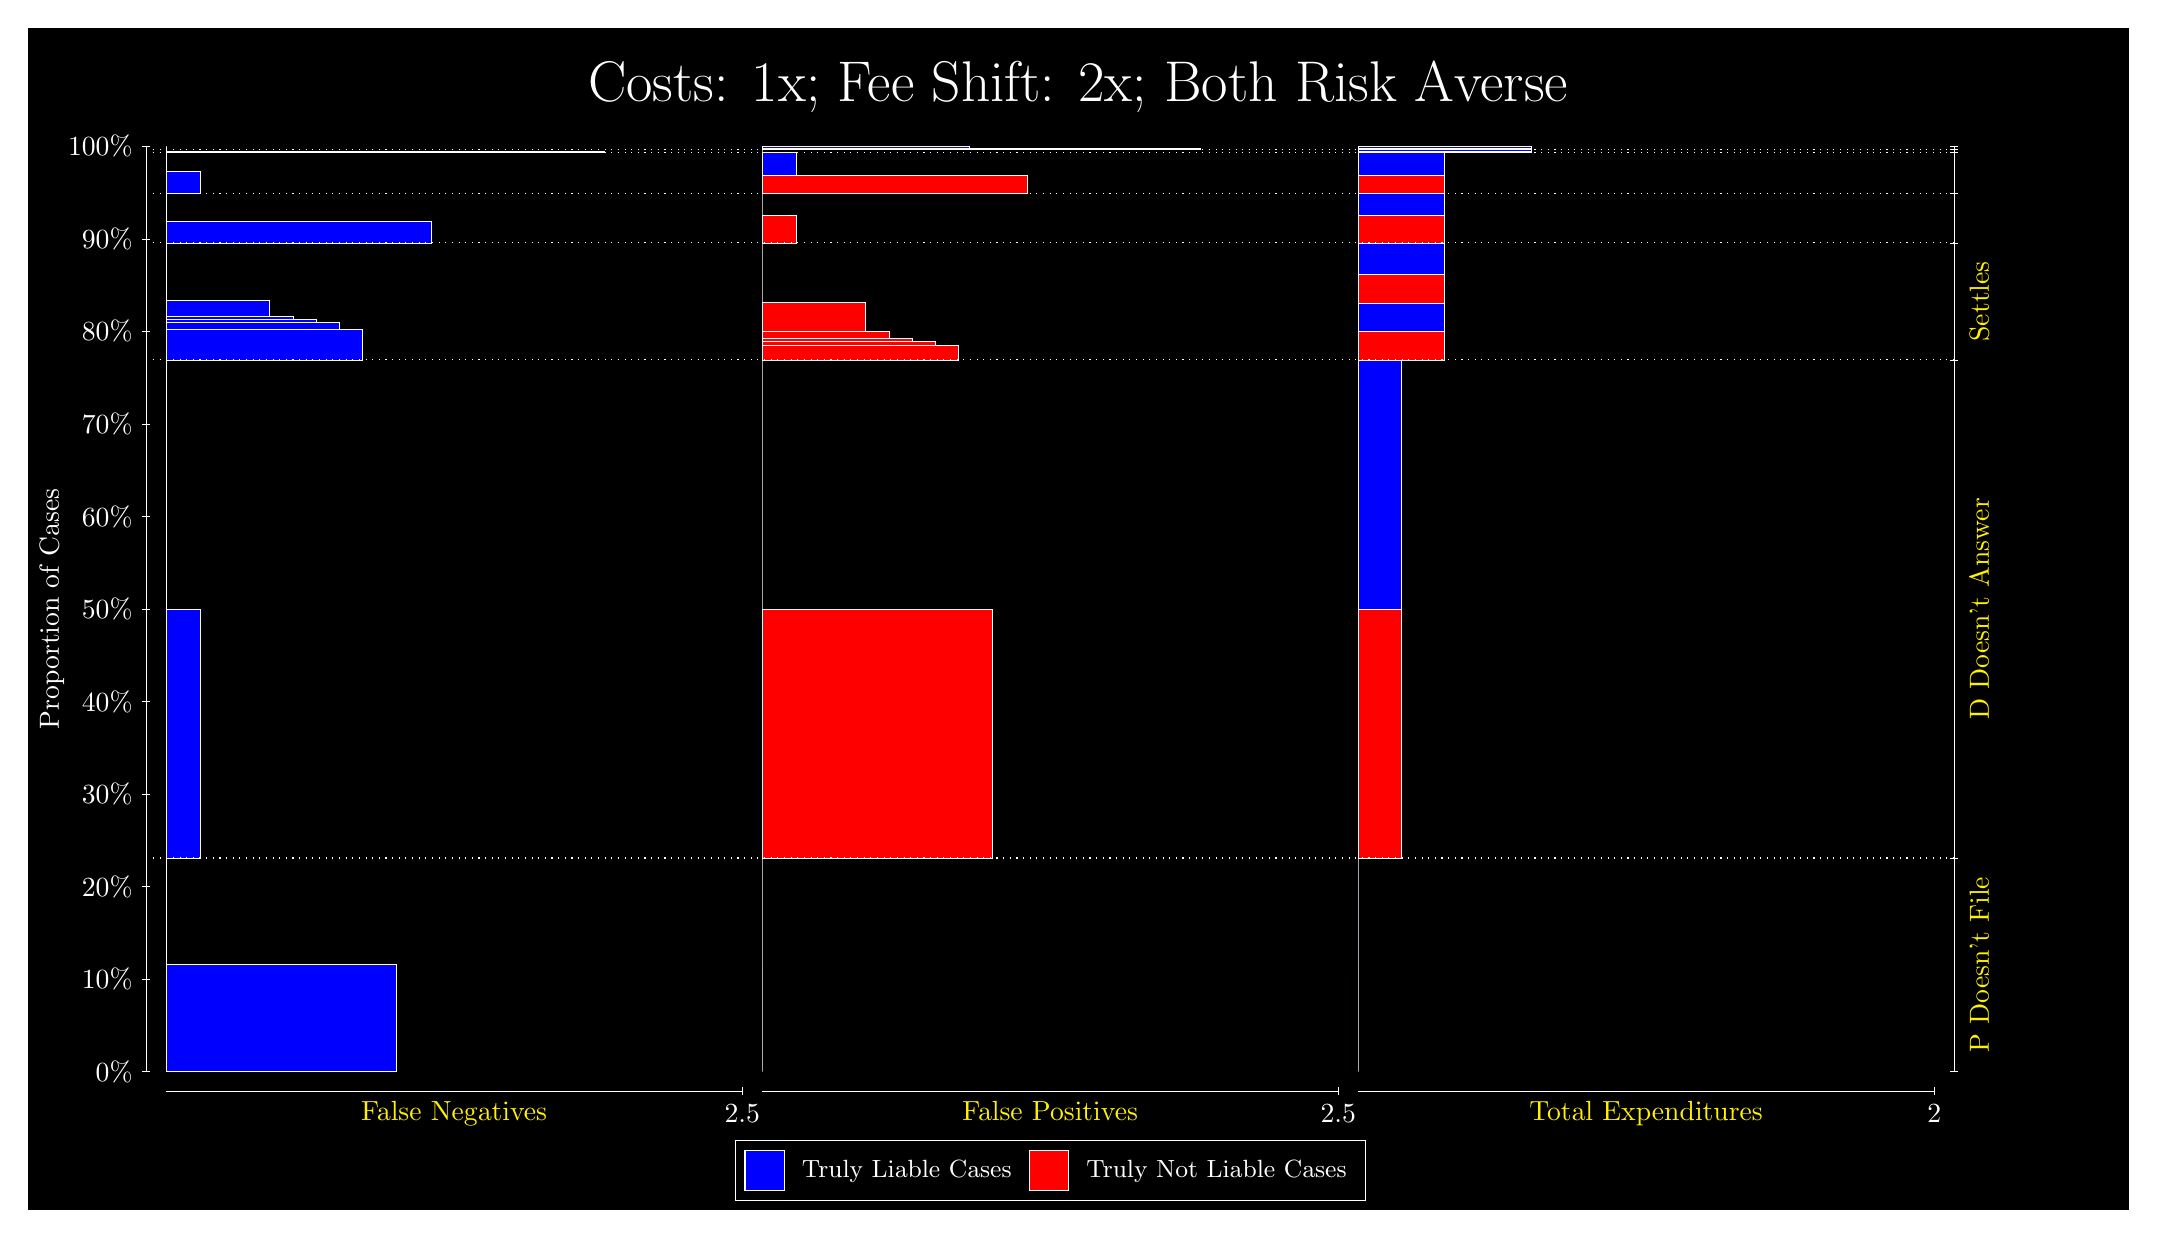
\begin{tikzpicture}
\draw[fill=black] (0,0) rectangle (26.667,15);
\draw[text=white] (0,13.5) rectangle (26.667,15) node[midway] {\huge Costs: 1x; Fee Shift: 2x; Both Risk Averse};
\draw[white, very thin] (1.5,1.75) -- (1.5,13.5);
\node[rotate=90, text=white, anchor=center] at (0.3, 7.625) {Proportion of Cases};
\draw[white, very thin] (1.45,1.75) -- (1.55,1.75);
\node[text=white, anchor=east] at (1.45, 1.75) {0\%};
\draw[white, very thin] (1.45,2.925) -- (1.55,2.925);
\node[text=white, anchor=east] at (1.45, 2.925) {10\%};
\draw[white, very thin] (1.45,4.1) -- (1.55,4.1);
\node[text=white, anchor=east] at (1.45, 4.1) {20\%};
\draw[white, very thin] (1.45,5.275) -- (1.55,5.275);
\node[text=white, anchor=east] at (1.45, 5.275) {30\%};
\draw[white, very thin] (1.45,6.45) -- (1.55,6.45);
\node[text=white, anchor=east] at (1.45, 6.45) {40\%};
\draw[white, very thin] (1.45,7.625) -- (1.55,7.625);
\node[text=white, anchor=east] at (1.45, 7.625) {50\%};
\draw[white, very thin] (1.45,8.8) -- (1.55,8.8);
\node[text=white, anchor=east] at (1.45, 8.8) {60\%};
\draw[white, very thin] (1.45,9.975) -- (1.55,9.975);
\node[text=white, anchor=east] at (1.45, 9.975) {70\%};
\draw[white, very thin] (1.45,11.15) -- (1.55,11.15);
\node[text=white, anchor=east] at (1.45, 11.15) {80\%};
\draw[white, very thin] (1.45,12.325) -- (1.55,12.325);
\node[text=white, anchor=east] at (1.45, 12.325) {90\%};
\draw[white, very thin] (1.45,13.5) -- (1.55,13.5);
\node[text=white, anchor=east] at (1.45, 13.5) {100\%};

\draw[white, very thin] (24.457,1.75) -- (24.457,13.5);
\draw[white, very thin] (24.407,1.75) -- (24.507,1.75);
\node[anchor=west] at (24.407, 1.75) {};
\draw[white, very thin] (24.407,4.4615) -- (24.507,4.4615);
\node[anchor=west] at (24.407, 4.4615) {};
\draw[white, very thin] (24.407,10.788) -- (24.507,10.788);
\node[anchor=west] at (24.407, 10.788) {};
\draw[white, very thin] (24.407,12.274) -- (24.507,12.274);
\node[anchor=west] at (24.407, 12.274) {};
\draw[white, very thin] (24.407,12.902) -- (24.507,12.902);
\node[anchor=west] at (24.407, 12.902) {};
\draw[white, very thin] (24.407,13.42) -- (24.507,13.42);
\node[anchor=west] at (24.407, 13.42) {};
\draw[white, very thin] (24.407,13.46) -- (24.507,13.46);
\node[anchor=west] at (24.407, 13.46) {};
\draw[white, very thin] (24.407,13.5) -- (24.507,13.5);
\node[anchor=west] at (24.407, 13.5) {};

\draw[white, very thin, fill=blue] (1.75,1.75) rectangle (4.6775,3.1058);
\draw[white, very thin, fill=red] (1.75,3.1058) rectangle (1.75,4.4615);
\draw[white, very thin, fill=blue] (1.75,4.4615) rectangle (2.1891,7.625);
\draw[white, very thin, fill=red] (1.75,7.625) rectangle (1.75,10.788);
\draw[white, very thin, fill=blue] (1.75,10.788) rectangle (4.2384,11.182);
\draw[white, very thin, fill=blue] (1.75,11.182) rectangle (3.9457,11.269);
\draw[white, very thin, fill=blue] (1.75,11.269) rectangle (3.6529,11.303);
\draw[white, very thin, fill=blue] (1.75,11.303) rectangle (3.3602,11.342);
\draw[white, very thin, fill=blue] (1.75,11.342) rectangle (3.0674,11.541);
\draw[white, very thin, fill=red] (1.75,11.541) rectangle (1.75,12.274);
\draw[white, very thin, fill=blue] (1.75,12.274) rectangle (5.1167,12.552);
\draw[white, very thin, fill=red] (1.75,12.552) rectangle (1.75,12.902);
\draw[white, very thin, fill=blue] (1.75,12.902) rectangle (2.1891,13.187);
\draw[white, very thin, fill=red] (1.75,13.187) rectangle (1.75,13.42);
\draw[white, very thin, fill=blue] (1.75,13.42) rectangle (7.3123,13.439);
\draw[white, very thin, fill=red] (1.75,13.439) rectangle (1.75,13.46);
\draw[white, very thin, fill=red] (1.75,13.46) rectangle (1.75,13.478);
\draw[white, very thin, fill=blue] (1.75,13.478) rectangle (1.75,13.5);
\draw[white, very thin, fill=red] (9.3189,1.75) rectangle (9.3189,3.1058);
\draw[white, very thin, fill=blue] (9.3189,3.1058) rectangle (9.3189,4.4615);
\draw[white, very thin, fill=red] (9.3189,4.4615) rectangle (12.246,7.625);
\draw[white, very thin, fill=blue] (9.3189,7.625) rectangle (9.3189,10.788);
\draw[white, very thin, fill=red] (9.3189,10.788) rectangle (11.807,10.975);
\draw[white, very thin, fill=red] (9.3189,10.975) rectangle (11.515,11.022);
\draw[white, very thin, fill=red] (9.3189,11.022) rectangle (11.222,11.06);
\draw[white, very thin, fill=red] (9.3189,11.06) rectangle (10.929,11.145);
\draw[white, very thin, fill=red] (9.3189,11.145) rectangle (10.636,11.522);
\draw[white, very thin, fill=blue] (9.3189,11.522) rectangle (9.3189,12.274);
\draw[white, very thin, fill=red] (9.3189,12.274) rectangle (9.758,12.624);
\draw[white, very thin, fill=blue] (9.3189,12.624) rectangle (9.3189,12.902);
\draw[white, very thin, fill=red] (9.3189,12.902) rectangle (12.686,13.135);
\draw[white, very thin, fill=blue] (9.3189,13.135) rectangle (9.758,13.42);
\draw[white, very thin, fill=red] (9.3189,13.42) rectangle (9.3189,13.442);
\draw[white, very thin, fill=blue] (9.3189,13.442) rectangle (9.3189,13.46);
\draw[white, very thin, fill=red] (9.3189,13.46) rectangle (14.881,13.478);
\draw[white, very thin, fill=blue] (9.3189,13.478) rectangle (11.954,13.5);
\draw[white, very thin, fill=red] (16.888,1.75) rectangle (16.888,3.1058);
\draw[white, very thin, fill=blue] (16.888,3.1058) rectangle (16.888,4.4615);
\draw[white, very thin, fill=red] (16.888,4.4615) rectangle (17.437,7.625);
\draw[white, very thin, fill=blue] (16.888,7.625) rectangle (17.437,10.788);
\draw[white, very thin, fill=red] (16.888,10.788) rectangle (17.986,11.145);
\draw[white, very thin, fill=blue] (16.888,11.145) rectangle (17.986,11.504);
\draw[white, very thin, fill=red] (16.888,11.504) rectangle (17.986,11.881);
\draw[white, very thin, fill=blue] (16.888,11.881) rectangle (17.986,12.274);
\draw[white, very thin, fill=red] (16.888,12.274) rectangle (17.986,12.624);
\draw[white, very thin, fill=blue] (16.888,12.624) rectangle (17.986,12.902);
\draw[white, very thin, fill=red] (16.888,12.902) rectangle (17.986,13.135);
\draw[white, very thin, fill=blue] (16.888,13.135) rectangle (17.986,13.42);
\draw[white, very thin, fill=red] (16.888,13.42) rectangle (19.083,13.442);
\draw[white, very thin, fill=blue] (16.888,13.442) rectangle (19.083,13.46);
\draw[white, very thin, fill=red] (16.888,13.46) rectangle (19.083,13.478);
\draw[white, very thin, fill=blue] (16.888,13.478) rectangle (19.083,13.5);
\draw[white, dotted] (1.5,4.4615) -- (24.457,4.4615);
\draw[white, dotted] (1.5,10.788) -- (24.457,10.788);
\draw[white, dotted] (1.5,12.274) -- (24.457,12.274);
\draw[white, dotted] (1.5,12.902) -- (24.457,12.902);
\draw[white, dotted] (1.5,13.42) -- (24.457,13.42);
\draw[white, dotted] (1.5,13.46) -- (24.457,13.46);
\draw[white, very thin] (1.75,1.5) -- (9.0689,1.5);
\node[text=yellow, anchor=north] at (5.4094, 1.5) {False Negatives};
\draw[white, very thin] (9.0689,1.45) -- (9.0689,1.55);
\node[text=white, anchor=north] at (9.0689, 1.45) {2.5};

\draw[white, very thin] (9.3189,1.5) -- (16.638,1.5);
\node[text=yellow, anchor=north] at (12.978, 1.5) {False Positives};
\draw[white, very thin] (16.638,1.45) -- (16.638,1.55);
\node[text=white, anchor=north] at (16.638, 1.45) {2.5};

\draw[white, very thin] (16.888,1.5) -- (24.207,1.5);
\node[text=yellow, anchor=north] at (20.547, 1.5) {Total Expenditures};
\draw[white, very thin] (24.207,1.45) -- (24.207,1.55);
\node[text=white, anchor=north] at (24.207, 1.45) {2};

\node[text=yellow, centered, rotate=90] at (24.777, 3.1058) {P Doesn't File};
\node[text=yellow, centered, rotate=90] at (24.777, 7.625) {D Doesn't Answer};
\node[text=yellow, centered, rotate=90] at (24.777, 11.531) {Settles};





\draw (12.978300999999998,1.5) node[draw=none] (baseCoordinate) {};
\begin{scope}[align=center]
        \matrix[scale=0.5, draw=white, below=0.5cm of baseCoordinate, nodes={draw}, column sep=0.1cm]{
            \node[rectangle, draw, minimum width=0.5cm, minimum height=0.5cm, fill=blue] {}; &
            \node[draw=none, font=\small, text=white] (B) {Truly Liable Cases}; &
            \node[rectangle, draw, minimum width=0.5cm, minimum height=0.5cm, fill=red] {}; &
            \node[draw=none, font=\small, text=white] (B) {Truly Not Liable Cases}; \\
            };
\end{scope}

\end{tikzpicture}
\end{document}